\chapter{Projektplanung}
\label{sec:Projektplanung}

\section{Gantt Chart}
F�r die Projektplanung wurde ein Java-Tool benutzt, welches auf dem Gantt-Diagramm basisert.\\
Ein Gantt-Diagramm oder Balkenplan ist ein nach dem Unternehmensberater Henry L. Gantt (1861?1919) benanntes Instrument des Projektmanagements, das die zeitliche Abfolge von Aktivit�ten grafisch in Form von Balken auf einer Zeitachse darstellt.\\

Quelle: \cite{gantt_chart}

\textcolor{red}{!!! IST DIES DEFINITIV ??? !!!}
\newpage
\begin{figure}[h]
\centering
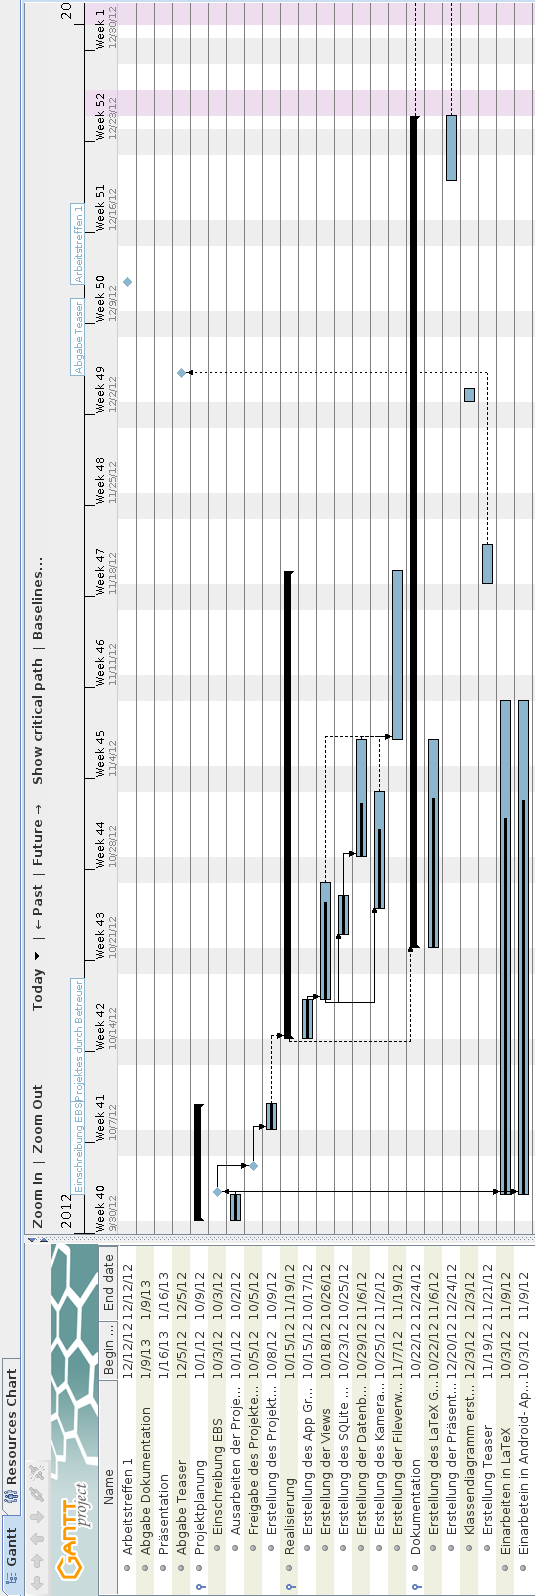
\includegraphics[height=17cm]{gantt_chart.png} \\
\caption{Gantt Chart Projekt Warranty}
\label{Gantt_Chart}
\end{figure}


\newpage
\section{Arbeitsaufw�nde}



\begin{tabular}[t]{|l|c|c|} \hline
\cellcolor{darkgrey} &  \cellcolor{darkgrey} &  \cellcolor{darkgrey}\\
\cellcolor{darkgrey} \multirow{-2}{5cm}{\textbf{Bezeichnung}} &
\cellcolor{darkgrey} \multirow{-2}{3cm}{\textbf{Aufwand gesch�tzt [h]}} &  
\cellcolor{darkgrey} \multirow{-2}{3cm}{\textbf{Aufwand effektiv [h]}}  \\ \hline

\multicolumn{3}{|l|}{} \\
\multicolumn{3}{|l|}{\multirow{-2}{5cm}{ \textbf{Projektplanung} }} \\ \hline
Ausarbeitung Projekdetails & 4 & 6 \\ \hline
Erstellung Projektplanes & 2 & 3 \\ \hline

\multicolumn{3}{|l|}{} \\
\multicolumn{3}{|l|}{\multirow{-2}{5cm}{ \textbf{Realisierung I} }} \\ \hline
Grundger�st Applikation  & 11 & \\ \hline
Views & 9 & \\ \hline
SQLite DB Schemas & 3 & \\ \hline
Datenbank Methoden & 6 & \\ \hline
Kamerasupports & 7  & \\ \hline
Fileverwaltung & 4 & \\ \hline


\multicolumn{3}{|l|}{} \\
\multicolumn{3}{|l|}{\multirow{-2}{5cm}{ \textbf{Realisierung II} }} \\ \hline
DB Zugriffe �berarbeiten  & 4 &  \\ \hline
File und Fotoverwaltung �berarbeiten & 3 & \\ \hline
Views �berarbeiten  &3 &  \\ \hline
Code Cleanup & 5 &  \\ \hline

\multicolumn{3}{|l|}{} \\
\multicolumn{3}{|l|}{\multirow{-2}{10cm}{ \textbf{Dokumentation und Pr�sentation} }} \\ \hline
Erstellung Teaser  & 3 & 2 \\ \hline
Erstellung Logo& 3 & 3 \\ \hline
Erstellung LaTeX Grundger�st  & 10 &  \\ \hline
1. Einleitung  & 3 &  \\ \hline
2. Projektplanung  & 3 &  \\ \hline
3. Grundlagen App Programmierung & 10 &  \\ \hline
4. Warranty App & 3 &  \\ \hline
5. Fazit & 3 &  \\ \hline
Anhang & 4 &  \\ \hline
Klassendiagramm & 3 &  \\ \hline
Erstellung Javadoc& 5 &  \\ \hline
Erstellung Pr�sentation & 12 &  \\ \hline

\multicolumn{3}{|l|}{} \\
\multicolumn{3}{|l|}{\multirow{-2}{10cm}{ \textbf{Diverses} }} \\ \hline
Einarbeitung in LATEX  & 15 & 26 \\ \hline
Einarbeitung Android Programming & 12 & 20 \\ \hline

&  &  \\
\textbf{Total Stunden}  & 
\textbf{150}&
\textbf{999}
\\ 

&  &  \\ \hline






\end{tabular}\\



